%
%  nietzsche.four
%
%  Created by Mark Eli Kalderon on 2008-02-24.
%  Copyright (c) 2008 Mark Eli Kalderon. All rights reserved.
%
%  Beamer

% Definitions and macros
\newcommand{\change}{\textcolor{blue}{\textbf{CHANGE SLIDE}}}
\newcommand\myauthor{Mark Eli Kalderon} 
\newcommand\mytitle{Introduction to Moral Philosophy}
\newcommand\mysubtitle{Nietzsche}
\newcommand\myinstitution{University College London}
\newcommand\myurl{http://markelikalderon.com/teaching}

% Packages specific to lecture notes
\mode<article>{
    \usepackage{palatino}
    \setjobnamebeamerversion{nietzsche.four.beamer}
}

% Packages specific to beamer presentation
\mode<presentation>{
    \usetheme{Darmstadt}
    \setbeamercovered{transparent}
    \pgfdeclareimage[height=0.5cm]{university-logo}{../../graphics/logo_sml_blk}
    \logo{\pgfuseimage{university-logo}}
}

% Packages common to lecture notes and beamer presentation
\usepackage{pgf}
\usepackage{tikz}
\usepackage{hyperref}

\title{\mytitle}
\subtitle{\mysubtitle}

\author{\myauthor\\
\url{\myurl}}
\institute{\myinstitution}

% \date[Short Occasion] % (optional)
% {Date / Occasion}

\begin{document}

\frame{\maketitle}

\change\ The second essay of the \emph{Genealogy} contains a subtle and complex discussion of the origin of guilt and bad conscience. My remarks in lecture will inevitably fail to do justice to the great wealth of ideas to be found in the second essay. What I hope to do, however, is to block out the main outlines of Nietzsche’s account of the contingent, historical processes that instilled in man not only the concept of a bad or guilty conscience but also the physiological mechanisms that implement it. The outline of the account is given by the upper left hand quarter of the genealogical tree in the handout I distributed. [Explain tree] \change

\begin{frame}<presentation>[label=slide1]
    \frametitle{Second Essay}
        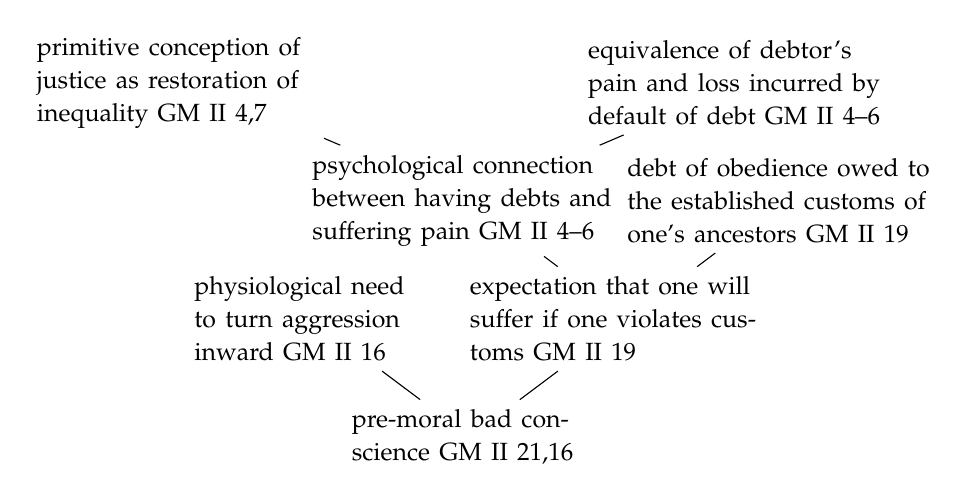
\begin{tikzpicture}
            \tikzstyle{level 1}=[sibling distance=4cm]
            \tikzstyle{level 2}=[sibling distance=4cm]
            \tikzstyle{level 3}=[sibling distance=7cm]
            \node[text width=3cm] {\small{pre-moral bad conscience GM II 21,16}} [grow'=up]
                child[text width=3cm] {node {\small{physiological need to turn aggression inward GM II 16}}}
                child {node[text width=4cm] {\small{expectation that one will suffer if one violates customs GM II 19}}
                    child {node[text width=4cm] {\small{psychological connection between having debts and suffering pain GM II 4--6}}
                        child {node[text width=4cm] {\small{primitive conception of justice as restoration of inequality GM II 4,7}}}
                        child {node[text width=4cm] {\small{equivalence of debtor's pain and loss incurred by default of debt GM II 4--6}}}}
                    child {node[text width=4cm] {\small{debt of obedience owed to the established customs of one's ancestors GM II 19}}}
                };
        \end{tikzpicture}
\end{frame}

Recall on Nietzsche's historicist version of interpretivism, interpreted practice has, in effect, a bipartite structure. There is a preexisting practice or form of life consisting of a distinctive set of actions, feelings, perceptions, beliefs and so on and an external will that gains mastery over and reinterprets this form of life. This contingent collision of a practice and a will that gains mastery over it and hence reinterprets it is represented in our diagram by branching nodes of the genealogical tree. Nietzsche's explicit statement of his brand of interpretivism and remarks concerning its relevance to historical methodology is to be found in sections 12 and 13 of the second essay.

Section 12 begins with a discussion of the genetic fallacy. How have previous genealogists accounted for the origin and meaning of punishment? Naively, according to Nietzsche, for they begin with the present function or value of punishment and then project that function or value back as the cause or origin of the institution of punishment. There is, however, no valid inference to be made from the present value of a thing to its causal origin, this is just the genetic fallacy. Nietzsche is resolute upon this point:
\begin{quote}
	However well one has understood the utility of any physiological organ (or of a legal institution, a social custom, a political usage, a form in art or in a religious art), this means nothing regarding its origin.
\end{quote}
Let us recall how the genetic fallacy is the central obstacle to providing an interpretation of the project of the \emph{Genealogy}. The \emph{Genealogy} is concerned with two questions: 
\begin{itemize}
	\item What is the value of our morality? 
	\item What are the conditions and circumstances that gave rise to our moral valuations? 
\end{itemize}
Nietzsche believes these questions to be related. In particular he thinks that in order to determine that value of our values we must first delineate the contingent. historical circumstances that gave rise to them. According to the genetic fallacy there is no direct inference from the value of a thing to its origin and vice versa. Given that Nietzsche explicitly criticizes previous genealogists for committing the genetic fallacy, it would be uncharitable in the extreme to attribute such a fallacy to him. Thus we have the central interpretive obstacle to reading the \emph{Genealogy}: what is the relation between determining the value of our values and determining the historical circumstances that gave rise to them?

As I remarked when we began the first essay, Nietzsche recommends the rigorous application of historical methods as a methodological corrective. That is, if one pays careful attention to the actual historical record, one will be less tempted to commit the genetic fallacy. Recall according to Nietzsche's interpretivism, an interpreted complex has a bipartite structure: he distinguishes that which is relatively enduring, a preexisting practice, and that which is fluid, the meaning or interpretation that has been projected onto that practice by an external will that gains mastery over it. It is precisely this doctrine that acts as a preventive, that forestalls the commission of the genetic fallacy. So for example, today a certain procedure or set of procedures involved in the institution of punishment have a certain purpose or utility these procedures are used for punishing. To claim that punishment, the procedures or set of procedures involved in the institution of punishment, was devised for punishing is to commit the genetic fallacy (since we have an inference from the present utility of these procedures to their origin). However, keeping clearly in mind the bipartite structure of an interpreted complex, a relatively enduring component, the preexisting practice and a fluid component, the interpretation imposed upon it by an external will, will forestall the commission of the genetic fallacy. It is not the case that the procedures involved in punishment were invented to discharge its present purpose, namely punishing. These procedures were not brought into being in order to subserve some function or purpose, rather they existed prior to the imposition of the function by a will that gained mastery over them. One methodological function of Nietzsche's historicist version of interpretivism is thus to insure that genealogist not commit the genetic fallacy. \change

I won't review in detail all of the features of Nietzsche's brand of interpretivism since I discussed them in an earlier lecture. But I do want to emphasize some points in relation to the distinction between forces and wills. Recall all struggles are conceived by Nietzsche to be conflicts between two or more unequal forces. A will is distinct from a force. A will is manifest in the contingent outcome of the struggle between opposing forces. The will is, in effect, the contingent synthesis of forces in opposition. Now when an agency gains mastery over some preexisting practice and thus reinterprets it, the interpretation that it imposes is not a function of the dominating force alone. The preexisting practice whether through inertia or active resistance will resist to some degree the force that seeks mastery over it. The interpretation that is imposed on the preexisting practice is thus the result of the dominating force and the partial success of counteractions on the part of the preexisting practice itself. Recall the will is not identified with the dominating force in a power struggle but rather with the contingent synthesis of the dominating force and the dominated force. Similarly an interpretation is not the product of the dominating force alone, but rather the dominating force together with the dominated force that resists it insofar as it can. Thus what interprets for Nietzsche is not dominating forces whether they be active or reactive. Rather what interprets is the will that is manifest in the contingent collision of opposing forces. \change

Recall, a will that successfully reinterprets a pre-existing practice by gaining mastery over it does not altogether obliterate whatever meaning it previously had. This has an important consequence. After successive episodes of reinterpretation by a variety of different wills, the meaning of a pre-exiting practice will be the contingent synthesis of not necessarily coherent meanings. As I emphasized in an earlier lecture, the result will be what Wittgenstein was later to describe as a family of resemblance concept: There will be no nontrivial feature that all and only things falling under that concept share---rather things that fall under that concept are sufficiently similar to one another in a number of different respects and there is no antecedently specifiable limit as to what counts as sufficient similarity. This is why Nietzsche claims that only that without a history may be defined---for a concept to have a definition is to have a set of non-trivial features that all and only things falling under that concept share. \change

\begin{frame}<presentation>[label=slide2]
    \frametitle{Interpretation and the Will}
        \begin{itemize}
            \item<1-> The distinction between a pre-existing practice and the interpretation that has been foisted upon it by some force that has gained mastery over it
            \item<2-> Given that a will is the contingent synthesis of forces in opposition it is the will that interprets
            \item<3-> Only that with no history has a definition  
        \end{itemize}
\end{frame}

One important early strand in the historical production of bad conscience is a primitive conception of justice where justice is understood as the restoration of equality. Thus if some injury or harm is done what is just according to this primitive conception is some means by which the harm is either undone or repaid in like kind. The well known Old Testament slogan, an eye for an eye, a tooth for a tooth is the expression of just this conception of justice. I have described this conception of justice which essentially involves the exchange of equivalents as a primitive conception of justice but it might better be described as a kind of proto-justice. Nietzsche believes that justice properly understood makes essential reference to a legal system in which it is embedded. But the historical origins of this sophisticated conception of justice involves the primitive conception of justice or proto-justice that Nietzsche believes evolved out of archaic commercial transactions. Commercial transactions originally involved the exchange of items of roughly equivalent value. Thus I might trade some of my goods for some your goods and the principle by which this transaction is negotiated is that we ought to exchange items of equivalent value. The primitive conception of justice is in effect a generalization of this principle governing archaic commercial transactions. Just as in barter one ought to strive for the exchange of rough equivalents, so in dealing with injury or harm, the recompense ought to be something that is equivalent to the injury or harm received. This can either take the form of restoring the harm incurred or it may take the more barbaric form or returning that harm in like kind.

In incurring harm or injury one is in effect a debtor owing some equivalent to the creditor, that is, the injured party.

The more sophisticated conception of justice is itself based on this principle governing archaic commercial transactions. Recall the sophisticated conception of justice is distinguished from its more primitive counterpart in that it is essentially embedded in a legal practice from which it gets its significance. On the sophisticated legalistic conception of justice, the person whom incurs some harm is still conceived to be a kind of debtor, but the debt is no longer owed to the injured party but rather the state or the legal system now assumes the role of the creditor. This reinterpretation of the primitive conception of justice is the result of some will, perhaps that of a primitive warlord, that established sovereignty through its greater strength. The will that overpowers a perhaps nomadic populace and establishes a state with a corresponding legal system has in a very real manner gained mastery over that populace as well as the primitive form of justice that it previously practiced. In so doing, not only has it gained sovereignty but has usurped the role of the creditor in matters of justice.

Both the primitive and legalistic conceptions of justice are generalizations of the principle governing archaic commercial transactions: that like should be exchanged for like. \change

\begin{frame}<presentation>[label=slide3]
    \frametitle{Primitive Conception of Justice}
        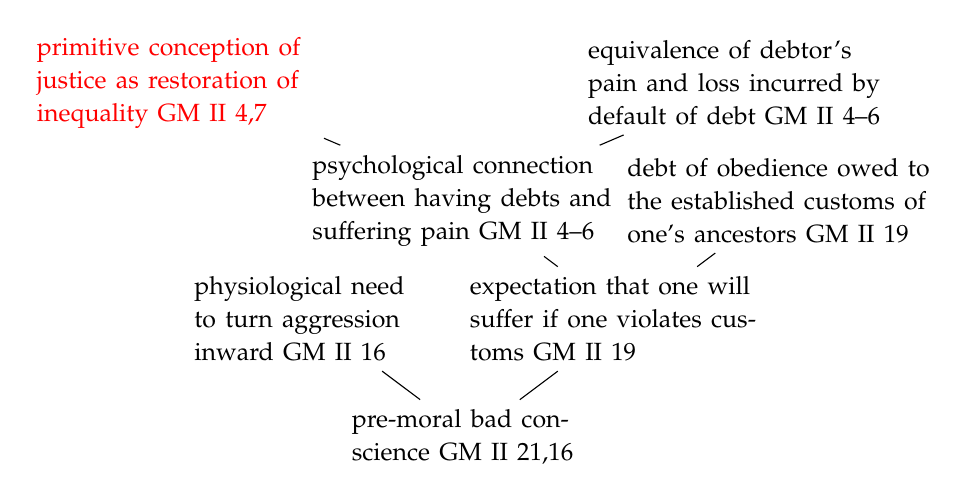
\begin{tikzpicture}
            \tikzstyle{level 1}=[sibling distance=4cm]
            \tikzstyle{level 2}=[sibling distance=4cm]
            \tikzstyle{level 3}=[sibling distance=7cm]
            \node[text width=3cm] {\small{pre-moral bad conscience GM II 21,16}} [grow'=up]
                child[text width=3cm] {node {\small{physiological need to turn aggression inward GM II 16}}}
                child {node[text width=4cm] {\small{expectation that one will suffer if one violates customs GM II 19}}
                    child {node[text width=4cm] {\small{psychological connection between having debts and suffering pain GM II 4--6}}
                        child {node[text=red,text width=4cm] {\small{primitive conception of justice as restoration of inequality GM II 4,7}}}
                        child {node[text width=4cm] {\small{equivalence of debtor's pain and loss incurred by default of debt GM II 4--6}}}}
                    child {node[text width=4cm] {\small{debt of obedience owed to the established customs of one's ancestors GM II 19}}}
                };
        \end{tikzpicture}
\end{frame}

There is a curious feature of archaic commercial transactions that is easily lost on moderns. Consider the situation where a debt is incapable of being discharged. Since the creditor has thus incurred a loss, the principle that such transactions ought to involve the exchange of equivalents has not been discharged. In such a case, the creditor can seek to discharge the debt by submitting the debtor to some terrible cruelty. Thus in Shakespeare's
``The Merchant of Venice'' Bassanio seeks to borrow three thousand ducats from Shylock the money lender with his friend Antonio as a guarantor of the debt. They agree to the following deal put to them by Shylock:
\begin{verse}
	This kindness will I show.\\
	Go with me to a notary, seal me there\\
	Your single bond; and, in merry sport,\\
	If you repay me not on such a day,\\
	In such a place, such sum or sums are\\ 
	Express'd in the condition, let the forfeit\\
	Be nominated for an equal pound\\
	Of your fair flesh, to be cut off and taken\\
	In what part of your body pleaseth me.\\
\end{verse}
Merry sport indeed. Notice the equivalent of three thousand ducats is deemed to be an equal pound of Antonio's fair flesh. Here again we see the principle governing archaic commercial transactions, namely, the exchange of equivalents. But in what sense is Antonio's mutilation in case of forfeiture equivalent to three thousand ducats of Shylocks money? Precisely in the \emph{merry sport} it will provide Shylock. It is the pleasure taken in this terrible act of cruelty which is exchanged for the three thousand ducats in case of forfeiture. When Antonio's shipping ventures fail one by one and forfeiture of the debt seems inevitable, Shylock is barely able to contain is glee for he will take great pleasure in taking his pound of flesh. This is but one example of the psychological willingness of archaic creditors to accept infliction of pain on a debtor as being in some sense equivalent to the loss incurred by default on a debt. What is perhaps difficult for we moderns to discern is the sense of the the equivalence. The pain inflicted on the debtor is equivalent to the loss incurred by forfeiture because of the pleasure the creditor will take in this cruel spectacle. However lest our more refined sensibilities make us incredulous at the prospect of the naked pleasure taken in cruelty I think we need only reflect on the schoolyard, that microcosm of human prehistory. Children readily take great pleasure in inflicting pain on one another. The bliss and innocence of childhood is a nostalgic myth, this is the dark lesson of the \emph{Lord of the Flies}. \change

\begin{frame}<presentation>[label=slide4]
    \frametitle{Debtor's Pain as Repayment}
        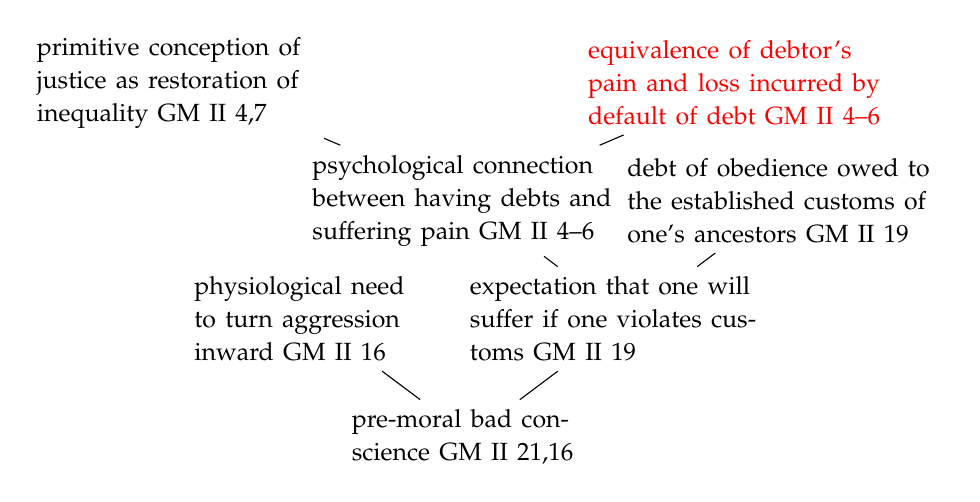
\begin{tikzpicture}
            \tikzstyle{level 1}=[sibling distance=4cm]
            \tikzstyle{level 2}=[sibling distance=4cm]
            \tikzstyle{level 3}=[sibling distance=7cm]
            \node[text width=3cm] {\small{pre-moral bad conscience GM II 21,16}} [grow'=up]
                child[text width=3cm] {node {\small{physiological need to turn aggression inward GM II 16}}}
                child {node[text width=4cm] {\small{expectation that one will suffer if one violates customs GM II 19}}
                    child {node[text width=4cm] {\small{psychological connection between having debts and suffering pain GM II 4--6}}
                        child {node[text width=4cm] {\small{primitive conception of justice as restoration of inequality GM II 4,7}}}
                        child {node[text=red,text width=4cm] {\small{equivalence of debtor's pain and loss incurred by default of debt GM II 4--6}}}}
                    child {node[text width=4cm] {\small{debt of obedience owed to the established customs of one's ancestors GM II 19}}}
                };
        \end{tikzpicture}
\end{frame}

So the governing principle of archaic commercial transactions had two important effects. First this principle that like must be exchanged for like was generalized beyond the realm of commerce to issue in a primitive conception of justice, a conception of justice succinctly and forcefully put in the Old Testament maxim, and eye for an eye and a tooth for a tooth. Second, the principle made possible the psychological disposition of some creditors to accept the infliction of pain on the debtor as being in some sense equivalent to the loss incurred by forfeiture of the debt. Together, in a contingent historical set of circumstances with this primitive conception of justice in play, as well as a creditor's willingness to accept the infliction of pain and the pleasure taken therein as equivalent to the debt owed, there was forged a certain psychological connection between having debts broadly construed and the expectation that one will suffer pain. To incur a debt, whether in commerce, or by harming one's fellow man, or by violating the laws that bind the state, now brought along with it the very real expectation that one will suffer pain.

With the establishment of this regular expectation that one will suffer having incurred a debt broadly construed, this dark foreboding of what will come unless the debt is properly discharged, we have the first important component of the mechanisms involved in a guilty conscience. \change

\begin{frame}<presentation>[label=slide5]
    \frametitle{Debts and the Expectation of Pain}
        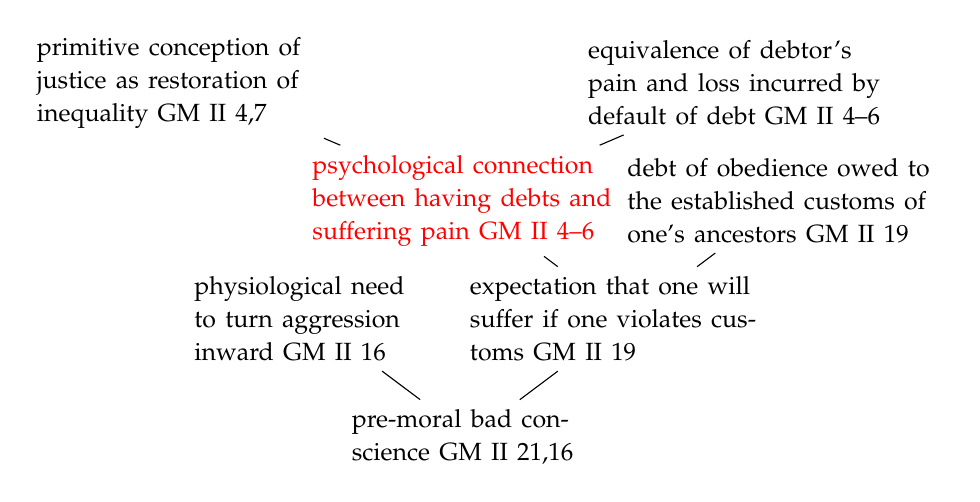
\begin{tikzpicture}
            \tikzstyle{level 1}=[sibling distance=4cm]
            \tikzstyle{level 2}=[sibling distance=4cm]
            \tikzstyle{level 3}=[sibling distance=7cm]
            \node[text width=3cm] {\small{pre-moral bad conscience GM II 21,16}} [grow'=up]
                child[text width=3cm] {node {\small{physiological need to turn aggression inward GM II 16}}}
                child {node[text width=4cm] {\small{expectation that one will suffer if one violates customs GM II 19}}
                    child {node[text=red,text width=4cm] {\small{psychological connection between having debts and suffering pain GM II 4--6}}
                        child {node[text width=4cm] {\small{primitive conception of justice as restoration of inequality GM II 4,7}}}
                        child {node[text width=4cm] {\small{equivalence of debtor's pain and loss incurred by default of debt GM II 4--6}}}}
                    child {node[text width=4cm] {\small{debt of obedience owed to the established customs of one's ancestors GM II 19}}}
                };
        \end{tikzpicture}
\end{frame}

Now this principle governing archaic commercial transactions, that like must be exchanged for like, was generalized not only to issue in a primitive conception of justice as well as a model for the relationship between a subjugated populace and the state that governs it, but was generalized as well to relationship one bore to one's ancestors. The founding fathers, as it were, of some primitive society were thought of as a kind of creditor. It is to one's ancestors that originally established the primitive society that one owed a debt for all the obvious advantages civil society provided over a nomadic lifestyle. To participate in civil society and enjoy its benefits was conceived to be indebted to one's ancestors who established that society. It is out of this further generalization of the structure of archaic commercial transactions that originated the idea that one owes the ancestors a debt of obedience to the customs they are thought to have established. How can this debt be discharge? The founding fathers are, after all, dead. The debt may be repaid by obedience to the customs they established. This, in effect, implements and propagates their will. \change

\begin{frame}<presentation>[label=slide6]
    \frametitle{Ancestor Worship}
        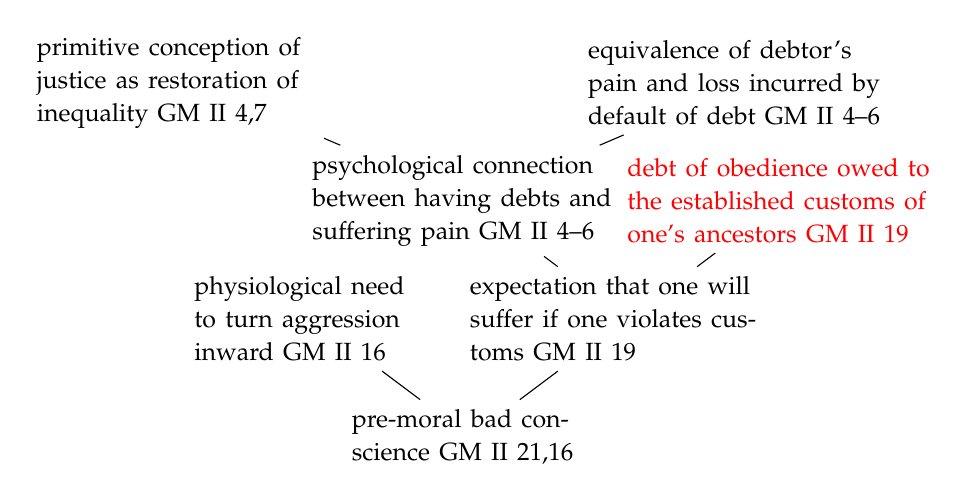
\begin{tikzpicture}
            \tikzstyle{level 1}=[sibling distance=4cm]
            \tikzstyle{level 2}=[sibling distance=4cm]
            \tikzstyle{level 3}=[sibling distance=7cm]
            \node[text width=3cm] {\small{pre-moral bad conscience GM II 21,16}} [grow'=up]
                child[text width=3cm] {node {\small{physiological need to turn aggression inward GM II 16}}}
                child {node[text width=4cm] {\small{expectation that one will suffer if one violates customs GM II 19}}
                    child {node[text width=4cm] {\small{psychological connection between having debts and suffering pain GM II 4--6}}
                        child {node[text width=4cm] {\small{primitive conception of justice as restoration of inequality GM II 4,7}}}
                        child {node[text width=4cm] {\small{equivalence of debtor's pain and loss incurred by default of debt GM II 4--6}}}}
                    child {node[text=red,text width=4cm] {\small{debt of obedience owed to the established customs of one's ancestors GM II 19}}}
                };
        \end{tikzpicture}
\end{frame}

Consider then, the contingent set of historical circumstances. Imagine some citizen of a primitive society. Our citizen enjoys obvious advantages over the nomadic lifestyle that is his only other recourse. And it is surely due to his ancestors that forged his society that he now enjoys such advantages. Furthermore commerce has provided a structural model for this relationship. He owes a debt to the ancestors for the advantages he presently enjoys. Furthermore, there is a regular expectation that one will suffer pain if one defaults on a debt. In such a historical condition there was thus forged the widespread psychological expectation that one will suffer if one violates the customs established by one's ancestors. \change

\begin{frame}<presentation>[label=slide7]
    \frametitle{Violation of Custom and the Expectation of Pain}
        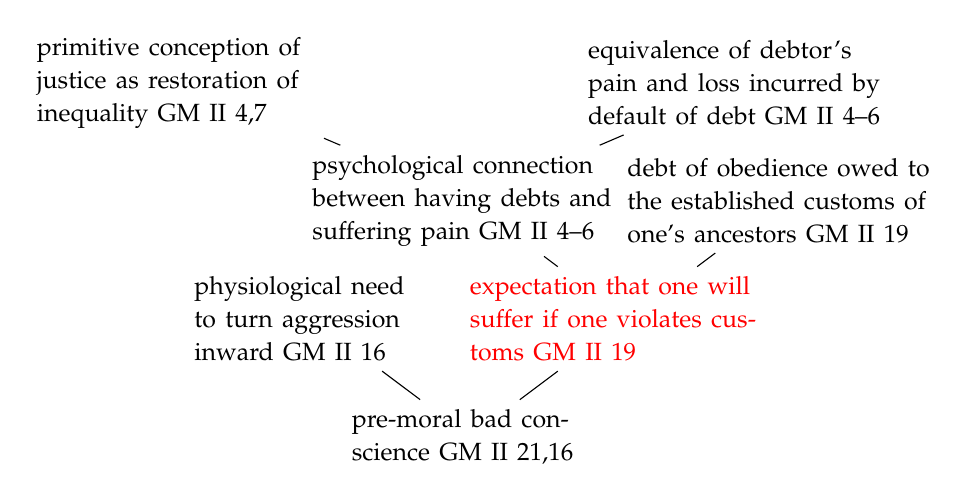
\begin{tikzpicture}
            \tikzstyle{level 1}=[sibling distance=4cm]
            \tikzstyle{level 2}=[sibling distance=4cm]
            \tikzstyle{level 3}=[sibling distance=7cm]
            \node[text width=3cm] {\small{pre-moral bad conscience GM II 21,16}} [grow'=up]
                child[text width=3cm] {node {\small{physiological need to turn aggression inward GM II 16}}}
                child {node[text=red,text width=4cm] {\small{expectation that one will suffer if one violates customs GM II 19}}
                    child {node[text width=4cm] {\small{psychological connection between having debts and suffering pain GM II 4--6}}
                        child {node[text width=4cm] {\small{primitive conception of justice as restoration of inequality GM II 4,7}}}
                        child {node[text width=4cm] {\small{equivalence of debtor's pain and loss incurred by default of debt GM II 4--6}}}}
                    child {node[text width=4cm] {\small{debt of obedience owed to the established customs of one's ancestors GM II 19}}}
                };
        \end{tikzpicture}
\end{frame}

Hopefully what is to eventually emerge, the mechanisms that implement a bad conscience, is coming more clearly into focus. There is yet another important element in the genealogy that leads to the establishment of the pre-moral bad conscience, that is the effects of urbanization on a previously nomadic populace. 

Nietzsche envisions the establishment of civil society as the imposition of a primitive warlord's will upon a previously nomadic populace. In subjugating a nomadic populace, the warlord imposes the form of civil society upon them. (This is a nice example of the qualitative feature of an active force, mentioned in a previous lecture---namely, that active forces are \emph{form-giving}.) The imposition of the form of civil society upon a previously nomadic populace had two important effects. 

The first has been mentioned earlier---that the primitive conception of justice, or proto-justice has been transformed. On the primitive conception of justice, the person who incurred harm was conceived to owe a debt to the person harmed. In subjugating a nomadic populace and establishing a legal system, the warlords reinterpret the primitive conception of justice and now conceive of the debt as being owed, not to the person harmed, but to the state. 

The second important effect was the eventual organization of the previously
nomadic populace in urban environments. This, according to Nietzsche, had an
important psychological effect. Formerly, all active instincts could be
immediately acted out. But with the imposition of civil society and the
accompanying urbanization, not all such instincts could be (on pin of
incurring a debt to the state) However, this active instinct, in being
so-constrained doesn't just disappear. The instinct continues to operate even if it can no longer operate on an external object. Nietzsche maintains that when an active force cannot be discharged externally, it is redirected inward. So the the psychological effect of urbanization is the physiological need to turn aggression inward.
\change

\begin{frame}<presentation>[label=slide8]
    \frametitle{Need to Turn Aggression Within}
        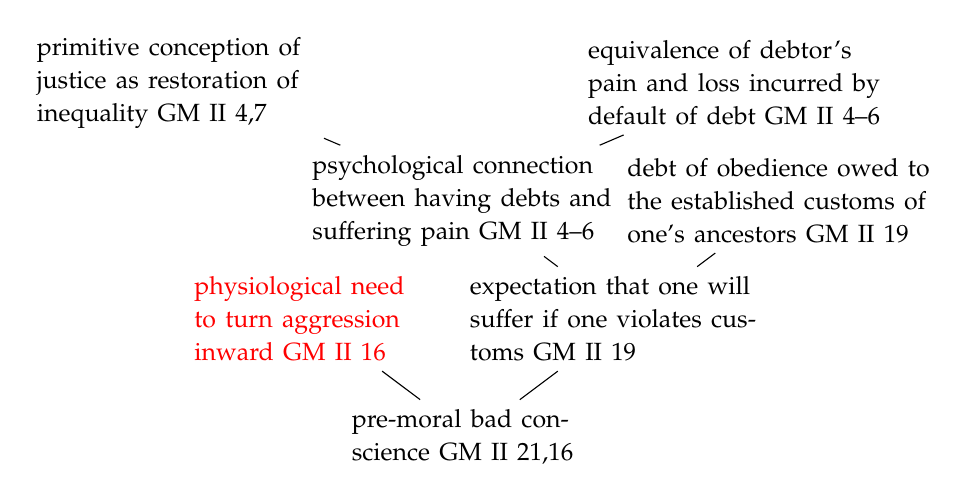
\begin{tikzpicture}
            \tikzstyle{level 1}=[sibling distance=4cm]
            \tikzstyle{level 2}=[sibling distance=4cm]
            \tikzstyle{level 3}=[sibling distance=7cm]
            \node[text width=3cm] {\small{pre-moral bad conscience GM II 21,16}} [grow'=up]
                child[text=red,text width=3cm] {node {\small{physiological need to turn aggression inward GM II 16}}}
                child {node[text width=4cm] {\small{expectation that one will suffer if one violates customs GM II 19}}
                    child {node[text width=4cm] {\small{psychological connection between having debts and suffering pain GM II 4--6}}
                        child {node[text width=4cm] {\small{primitive conception of justice as restoration of inequality GM II 4,7}}}
                        child {node[text width=4cm] {\small{equivalence of debtor's pain and loss incurred by default of debt GM II 4--6}}}}
                    child {node[text width=4cm] {\small{debt of obedience owed to the established customs of one's ancestors GM II 19}}}
                };
        \end{tikzpicture}
\end{frame}

Active forces are form giving. The subjugation of a nomadic populace by some band of warlords is the exercise of an active force in its crudest from. But it is also form-giving in the sense that the subjugation of the populace imposes upon them the form of civil society. Similarly the active forces turned inward because of the results of urbanization are themselves form-giving. Instead of imposing a form on others, these forces impose a form on man himself. 

The presence of a need to turn aggression inwards operates in a contingent historical circumstance where there is an expectation that one will suffer if one violates the customs established by one's ancestor's. An effect of this is that when one violates an established custom, one's expectation of pain will be fulfilled by the flood of violent emotion that is the result of turning aggression inward. If one violates the moral code one will under those conditions be disposed to feel guilty.

Punishment plays a role in the establishment of civil society. Punishment precedes and is the cause of bad conscience and gilt. The procedures involved in punishment were not invented to punish the guilty. (To suppose otherwise would be to commit the genetic fallacy.) Rather, punishment in effect invented guilt

Guilt and bad canscience are not necessarily bad despite their cruel prehistory. Nietzsche considers them to be a remarkbale achievement and one that could be used to promote human flourishing of this new animal type man. Thus his discussion of the autonomous agent with the right to make promises.

The bad conscience may also be used by a negative will and hinder human flourishing. This, Nietzsche contends, is what happens with the moralizing misinterpretation of the bad conscience imposed by the priestly will of Paul. We will return to this when we discuss the third essay.\change

\begin{frame}<presentation>[label=slide9]
    \frametitle{Pre-Moral Bad Conscience}
        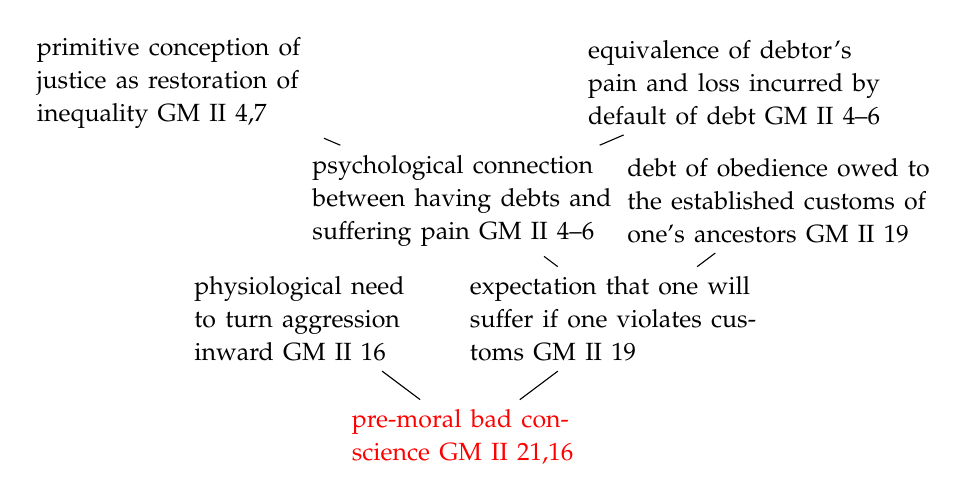
\begin{tikzpicture}
            \tikzstyle{level 1}=[sibling distance=4cm]
            \tikzstyle{level 2}=[sibling distance=4cm]
            \tikzstyle{level 3}=[sibling distance=7cm]
            \node[text=red,text width=3cm] {\small{pre-moral bad conscience GM II 21,16}} [grow'=up]
                child[text width=3cm] {node {\small{physiological need to turn aggression inward GM II 16}}}
                child {node[text width=4cm] {\small{expectation that one will suffer if one violates customs GM II 19}}
                    child {node[text width=4cm] {\small{psychological connection between having debts and suffering pain GM II 4--6}}
                        child {node[text width=4cm] {\small{primitive conception of justice as restoration of inequality GM II 4,7}}}
                        child {node[text width=4cm] {\small{equivalence of debtor's pain and loss incurred by default of debt GM II 4--6}}}}
                    child {node[text width=4cm] {\small{debt of obedience owed to the established customs of one's ancestors GM II 19}}}
                };
        \end{tikzpicture}
\end{frame}
\section*{Summary}

\end{document}
